\section{Assumptions of survival analysis}

%----------------------------------------------------------------------
\begin{frame}{Common assumptions in survival analysis}
    \begin{enumerate}
    \item Subjects are \textbf{either} ``healthy'' \textbf{or}
      ``diseased'', with no intermediate state.
    \item The disease is \textbf{irreversible}, or requires
      intervention to be cured.
    \item The time of disease incidence is known \textbf{exactly}.
    \item The disease is \textbf{accurately} diagnosed.
    \end{enumerate}
    \pause
    These assumptions are true for \alert{death} and many
    \alert{chronic diseases}.
    \pause
    
    A question of definition:\\ -- consider occurrence of \textbf{recording of} a
    given disease
\end{frame}

% %----------------------------------------------------------------------
% \begin{frame}{Is the disease a dichotomy?}
%   A disease may be preceded by a \alert{sub-clinical} phase before it shows
%   symptoms.
%   \pause
%   \begin{center}
%     \begin{tabular}{ll}
%       {\bf AIDS} & Decline in CD4 count \\
%       {\bf Cancer} & Pre-cancerous lesions \\
%       {\bf Type 2 Diabetes} & Impaired glucose tolerance \\
%     \end{tabular}
%   \end{center}
%   \pause
%   Or a disease may be classified into \alert{degrees of severity}
%   (mild, moderate, severe).
% \end{frame}

%----------------------------------------------------------------------
\begin{frame}{A model for cervical cancer}
  Invasive squamous cell cancer of the cervix is preceded by
  cervical intraepithelial neoplasia (CIN)\\[-1.5em]
%\hspace*{-1em}
\includegraphics<1-2|handout:0>[width=1.1\textwidth,keepaspectratio]{cervical2}
\includegraphics<3|handout:0>[width=1.1\textwidth,keepaspectratio]{cervical3}
\includegraphics<4-|handout:1>[width=1.1\textwidth,keepaspectratio]{cervical4}\\[-1.5em]

\pause Purpose of a screening programme is to detect and treat
CIN --- status of persons obtained at screening dates

\pause \alert<5->{Aim} of the modeling the \alert<3>{transition rates}
  between \alert<4>{states},
  is to be able predict how population moves between
  \alert<4>{states}
  
\pause \pause 
  \begin{itemize}
    \item Transition rates between states
    \item Probability of state occupancy
  \end{itemize}
\end{frame}

% %----------------------------------------------------------------------
% \begin{frame}
%   \frametitle{When does the disease occur?}

%   You may need a \alert{clinical visit} to diagnose the disease:
%   \begin{itemize}[<+->]
%     \item examination by physician, or
%     \item laboratory test on blood sample, or
%     \item examination of biopsy by pathologist
%   \end{itemize}
%   \pause
%   We do not know what happens between consecutive visits\\ (interval
%   censoring).

% \end{frame}

% %----------------------------------------------------------------------
% \begin{frame}
%   \frametitle{Informative observation process?}

%   Is the \textbf{reason} for the visit dependent on the \textbf{evolution}
%   of disease?

%   \pause
%   Ignoring this may cause bias, like informative censoring.

%   \pause
%   Different reasons for follow-up visits:
%   \begin{itemize}
%     \item Fixed intervals (OK)
%     \item Random intervals (OK)
%     \item Doctor's care (OK)
%     \item Self selection (\textbf{Not} OK --- visits are likely to be
%       close to event times)
%   \end{itemize}

% \end{frame}

% %----------------------------------------------------------------------
% \begin{frame}
%   \frametitle{Do We Know The True Disease State?}

%   \begin{itemize}
%     \item Biomarkers may have \alert{random error}
%     \item Correct diagnosis may require \alert{invasive} procedure
%       \begin{itemize}
% 	\item Cytology vs histology for CIN.
%       \end{itemize}
%     \item Inter-rater \alert{disagreement}
%       \begin{itemize}
% 	\item Accurate diagnosis may require a consensus panel.
%       \end{itemize}
%   \end{itemize}

% \end{frame}

% \section{Introducing Multi-State Models}

% %----------------------------------------------------------------------
% \begin{frame}{Multistate  Terminology}
%   We can convert (some) terminology from survival analysis:
%   \pause
%   \begin{center}
%   \begin{tabular}{lcl}
%   Case status              & $\rightarrow$ & (Disease) state \\
%   Disease Incidence        & $\rightarrow$ & Transition (between states) \\
%   Incidence/mortality rate & $\rightarrow$ & Transition intensities \\
%   \end{tabular}
%   \end{center}
%   \begin{center}
%   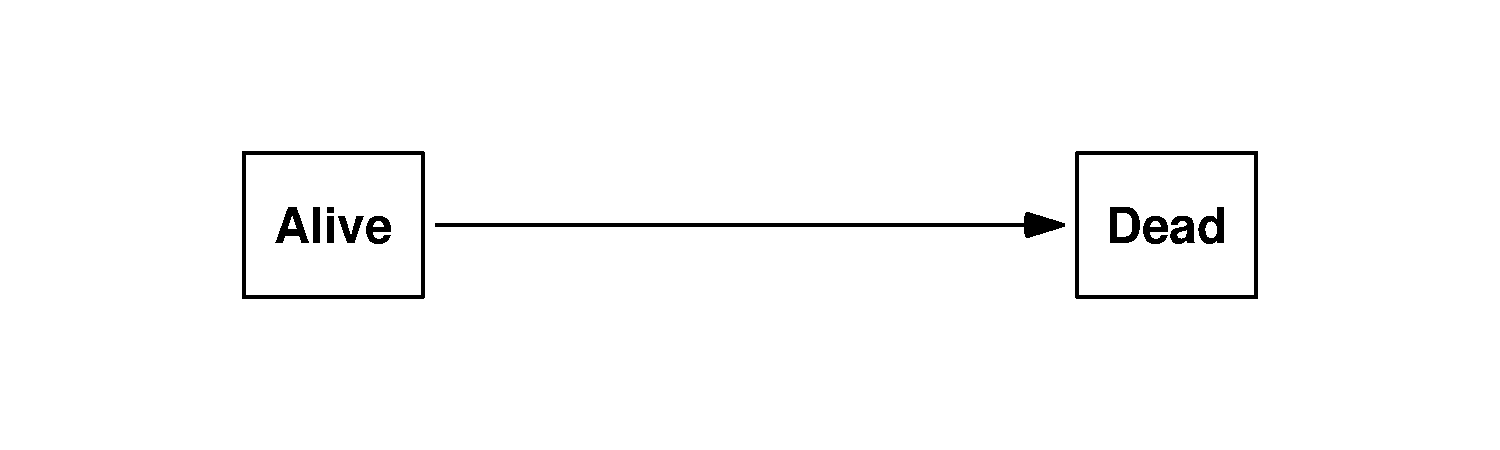
\includegraphics[width=\textwidth,keepaspectratio]{simple-surv}
%   \end{center}
% \end{frame}

%----------------------------------------------------------------------
\begin{frame}{Markov models for multistate processes}
  The natural generalization of Poisson regression to multiple
    disease states:
  \pause
    \begin{itemize}
    \item transition between states depends \textbf{only} on current state
    \item --- this is the \textbf{Markov} property
    \item $\Rightarrow$ transition rates are constant over time
    \item (time-fixed) covariates may influence transition rates
    \item the formal Markov property is \textbf{very} restrictive
    \item in the clinical litterature ``Markov model'' is often used
      about any type of multistate model
    \end{itemize}
\end{frame}

% %----------------------------------------------------------------------
% \begin{frame}{An Illness-Death Model}
% \vspace*{-1em}
% \hspace*{-2em}
% 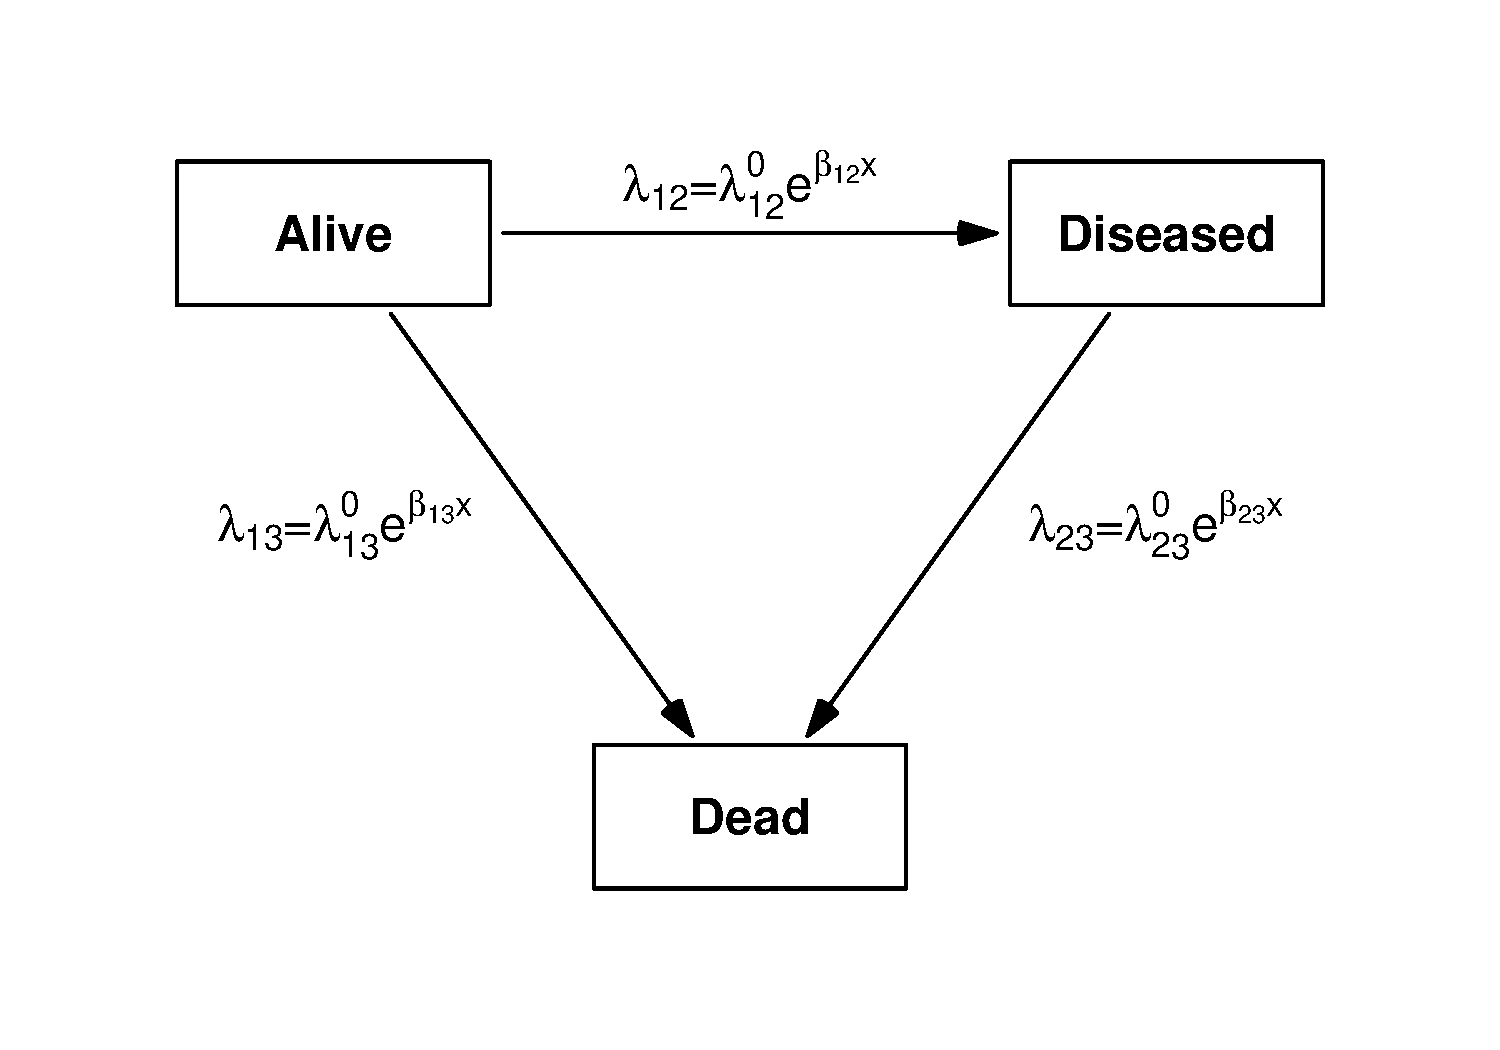
\includegraphics[height=0.85\textheight,keepaspectratio]{ill-death}\\[-1ex]
% Note: Constant transition intensities between states
% \end{frame}

%----------------------------------------------------------------------
\begin{frame}{Components of a multistate (Markov) model}
  \begin{itemize}
    \item Define the disease states
    \item Define which transitions between states are allowed
    \item Select covariates influencing transition rates (may be
      different between transitions)
    \item Not a trivial task --- do we want \textit{e.g.}

      \begin{itemize}
      \item cause of death (CVD, Cancer, Other)
      \item disease status at death (prev.CVD, prev.Can, neither)
      \end{itemize}

  \end{itemize}
\end{frame}

%----------------------------------------------------------------------
\begin{frame}{A more complicated multistate model}
\vspace*{-1em}
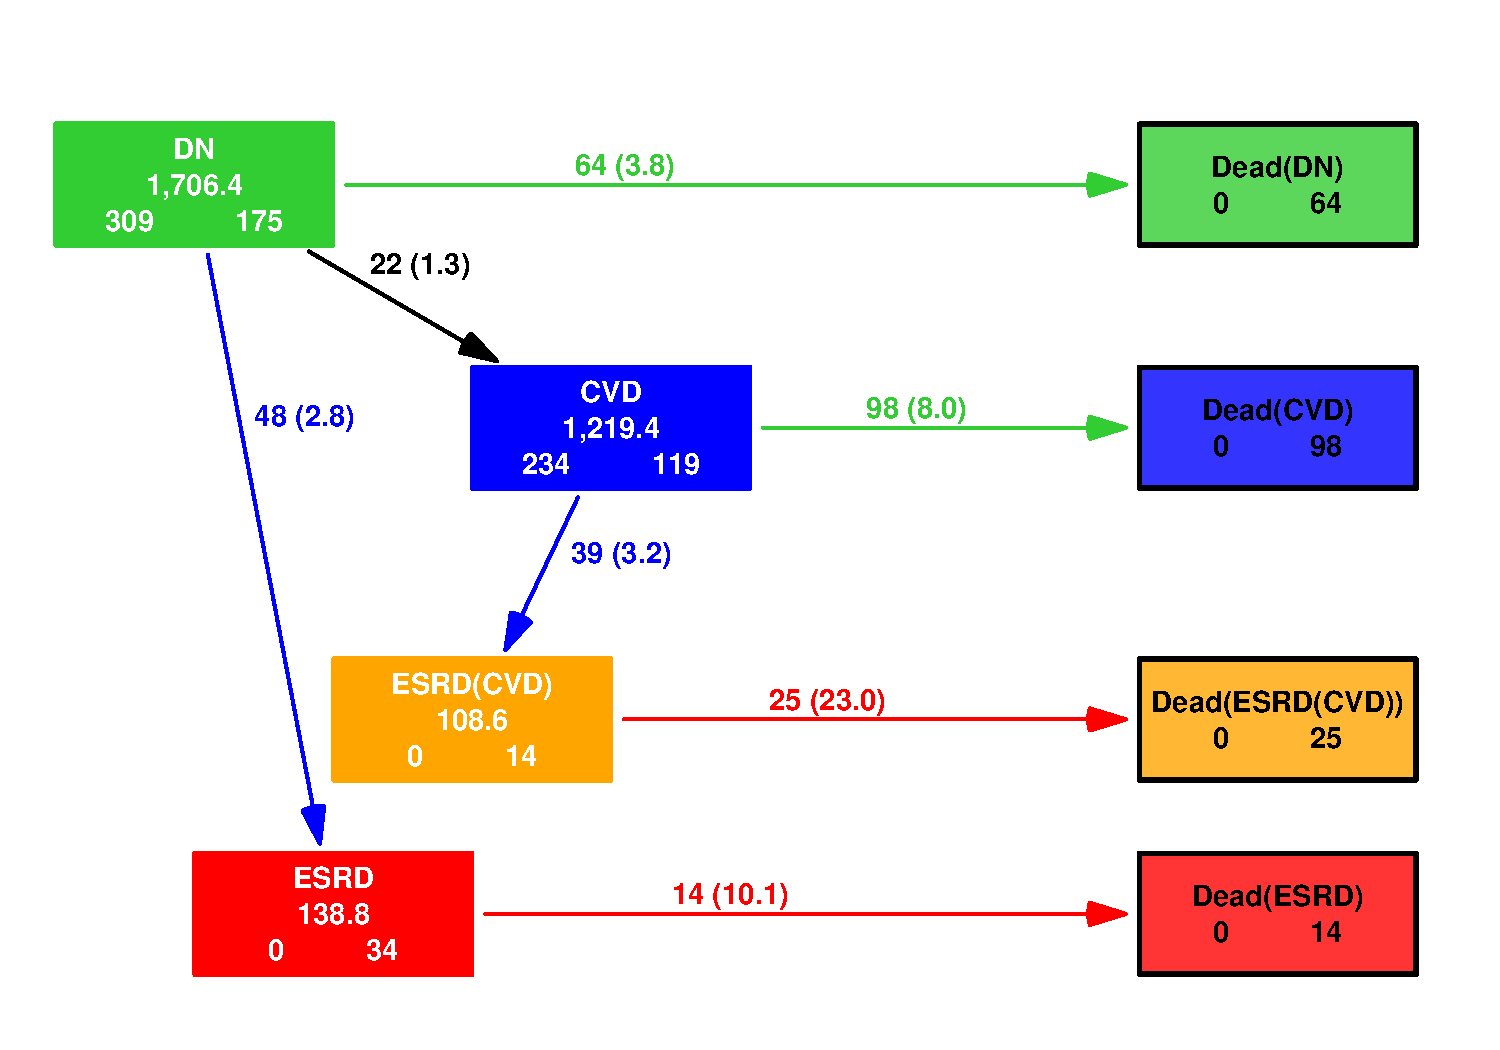
\includegraphics[width=0.82\textwidth]{./GbAd-states.pdf}
\end{frame}

\section{Defining Multi-State Markov Models}

% %----------------------------------------------------------------------
% \begin{frame}{Formal definition}
%   A model is defined by its \alert{transition intensity matrix}
%   \[
%   Q = \left(
%   \begin{array}{@{\extracolsep{1em}}ccc}
%     -\lambda_{12}  - \lambda_{13} & \lambda_{12}  & \lambda_{13} \\
%     0                            & -\lambda_{23} & \lambda_{23} \\
%     0                            & 0            &  1 \\
%   \end{array}
%   \right)
%   \]
%   \vspace*{-1em}
%   \pause
%   \begin{itemize}
%   \item Off-diagonal elements are instantaneous transition rates
%     (or intensities) between two different states.
%   \item If states are ordered by severity:

%     \begin{itemize}
%     \item Above the diagonal = progression
%     \item Below the diagonal = regression
%     \end{itemize}

%   \item Diagonal elements are fixed by the constraint that rows of $Q$
%     sum to zero.
%   \end{itemize}
% \end{frame}

%  %----------------------------------------------------------------------
% \begin{frame}{Likelihood for a Markov model}
%   \begin{itemize}
%   \item The likelihood of the model depends on the probability of being in
%     state $j$ at time $t_1$, given that you were in state $i$ at time $t_0$.
%   \item This is given by $P_{ij}$ where
%     \[
%     P = \exp(Q(t_1 - t_0))
%     \]
%   \item The \alert{matrix exponential} is hard to calculate (from a
%     numerical point of view).
%   \item \textbf{Only} refers to transition rates that are constant in time.
%   \end{itemize}
% \end{frame}

% %----------------------------------------------------------------------
% \begin{frame}
%   \frametitle{Covariate Effects are Multiplicative}

%   For an individual $i$ with risk factors $z_i$
%   \[
%   \lambda^i_{jk} = \lambda^0_{jk} \times \exp(\beta_{jk}^T z^i)
%   \]
%   There is a separate baseline rate hazard ratio for each possible
%   transition.
% \end{frame}

% %----------------------------------------------------------------------
% \begin{frame}
%   \frametitle{Hidden Markov Models}

%   For cases where the disease process is observed indirectly.
%   \pause
%   We have:
%   \begin{itemize}[<+->]
%   \item A possibly misclassified diagnosis, or
%   \item An indirect surrogate of disease status.
%   \end{itemize}
%   \pause
%   Add a \alert{measurement model} to describe the relation between
%   true and observed state.
%   \[
%   \mbox{P}(\mbox{Observed state} \mid \mbox{True state})
%   \]
% \end{frame}

%----------------------------------------------------------------------
\begin{frame}{Likelihood for a multistate model}
  \begin{itemize}
  \item The likelihood of the model depends on the probability of
    being in state \texttt{B} at time $t_1$, given that you were in
    state \texttt{A} at time $t_0$.
  \item Assume transition rates constant in small time intervals,
    $\lambda^{\mathtt{A}\rightarrow\mathtt{B}}$
  \item $\Rightarrow$ each interval for a person contributes term(s)
    to the likelihood
  \item one term for each possible transition to a subsequent state
  \item the total log-likelihood for person $p$ in state \texttt{A}
    during interval $i$ is a
    sum of these terms:
    \alert<6>{$\ell_p = \sum_{i,\mathtt{B}}d_{pi}\big(
      \log(\lambda^{\mathtt{A}\rightarrow\mathtt{B}}_{pi})-
           \lambda^{\mathtt{A}\rightarrow\mathtt{B}}_{pi}y_{pi}\big)$}
  \item $\Rightarrow$ each term has the form of the likelihood for a\\
    Poisson variate \alert<6>{$d$} with mean \alert<6>{$\lambda y$}
  \end{itemize}
\end{frame}

%----------------------------------------------------------------------
\begin{frame}{Likelihood for a multistate model}
  \begin{itemize}
    \item each term has the form of the likelihood for a Poisson
      variate $d$ with mean $\lambda y$
  \item terms are \textbf{not} independent, but the total
    likelihood is a product; hence of the same form as the
    likelihood from independent Poisson variates
  \item but observations from intervals from one person are\\
    neither Poisson nor independent
  \end{itemize}
\end{frame}

%----------------------------------------------------------------------
\begin{frame}{Realms of multistate modeling}
  \begin{itemize}
  \item intensities --- dimension \alert<4>{$\textrm{time}^{-1}$}\\
    this is the scale of observation, $(d,y)$ (complete data)
  \item state probabilities --- dimensionless, \alert<4>{$\textrm{time}^{0}$}\\
    \alert<4>{integral} of intensities w.r.t. to time
  \item sojourn times --- dimension \alert<4>{$\textrm{time}^{1}$}\\ 
    \alert<4>{integral} of state probabilities w.r.t. to time
  \end{itemize}
\end{frame}

%----------------------------------------------------------------------
\begin{frame}{Classes of multistate models}
  \begin{itemize}
  \item Markov model: transition between states depends \textbf{only}
    on current state $\Rightarrow$ transition rates are constant\\
    \alert<5->{time-homogeneous Markov model}
  \item If transition rates depend on the \textbf{same timescale}
    only we have a \alert<5->{time-\textbf{in}homogeneous Markov model}
  \item If transition rates depend on the time since entry to the
    current state we have a \alert<5->{\textbf{semi}-Markov model}
  \item If transition rates depend on several timescales we have a
    \alert<5->{general multistate model} (there is no formal name for this)
  \end{itemize}
  \pause
  \ldots it is common-place in the literature to use the term ``Markov
  model'' for any type of multistate model.
\end{frame}

%----------------------------------------------------------------------
\begin{frame}{Computing state probabilities\newline from intensities in multistate models}
  \begin{itemize}
  \item time-homogeneous Markov model:\\closed-form formulae exist 
  \item time-\textbf{in}homogeneous Markov model:\\closed-form
    formulae exist (a bit more complicated)
  \item \textbf{semi}-Markov model:\\no closed form formulae exist  
  \item general multistate model:\\no closed form formulae exist  
  \end{itemize}
  \pause
  No formulae means that any inference on state probabilities and sojourn
  times must be based on \textbf{simulation} from the model.
\end{frame}

